\documentclass[../thesis/thesis.tex]{subfiles}
\begin{document}
 \chapter{Sensor Properties}

%\afterpage{\global\pdfpageattr\expandafter{\the\pdfpageattr/Rotate 90}}
\begin{sidewaystable}
{\small
\begin{tabular}{*{16}{|z{2.5em}}|}
\hline
14.95 0.51 & 14.33 0.27 & 12.34 0.27 & 8.77 0.33 & 8.15 0.31 & 10.84 0.38 & 9.02 0.26 & 7.79 0.37 & 6.67 0.27 & 9.63 0.29 & 9.29 0.26 & 8.24 0.27 & 9.84 0.25 & 14.28 0.33 & 14.92 0.3 & 13.16 0.25 \\ \hline
14.54 0.34 & 15.62 0.31 & 12.73 0.23 & 11.51 0.27 & 11.79 0.26 & 11.47 0.27 & 11.43 0.29 & 9.02 0.35 & 8.57 0.23 & 11.15 0.23 & 10.64 0.22 & 10.3 0.24 & 12.09 0.22 & 14.49 0.26 & 14.88 0.31 & 14.71 0.36 \\ \hline
18.25 0.45 & 16.62 0.31 & 14.15 0.24 & 11.97 0.34 & 13.11 0.3 & 12.64 0.22 & 10.66 0.23 & 9.15 0.24 & 9.58 0.28 & 11.95 0.28 & 11.22 0.24 & 11.52 0.36 & 11.11 0.23 & 12.59 0.25 & 14.44 0.31 & 13.35 0.28 \\ \hline
16.02 0.28 & 16.81 0.36 & 15.0 0.25 & 11.53 0.28 & 10.18 0.29 & 12.2 0.25 & 11.78 0.29 & 8.36 0.31 & 8.15 0.33 & 10.36 0.32 & 10.74 0.31 & 8.25 0.36 & 9.99 0.35 & 12.42 0.38 & 11.39 0.4 & 11.06 0.34 \\ \hline
\end{tabular}
}
\caption{Mean and standard deviations for each pixel at rest}
\label{tab:meanstd}
\end{sidewaystable}
%\afterpage{\global\pdfpageattr\expandafter{\the\pdfpageattr/Rotate 0}}

In \Fref{tab:meanstd} the thermal sensor was exposed to the night sky at a capture rate of 1Hz for 4 minutes, with the sensing results combined to create a set of means and standard deviations to indicate the pixels at ``rest''.


\begin{figure}
\centering
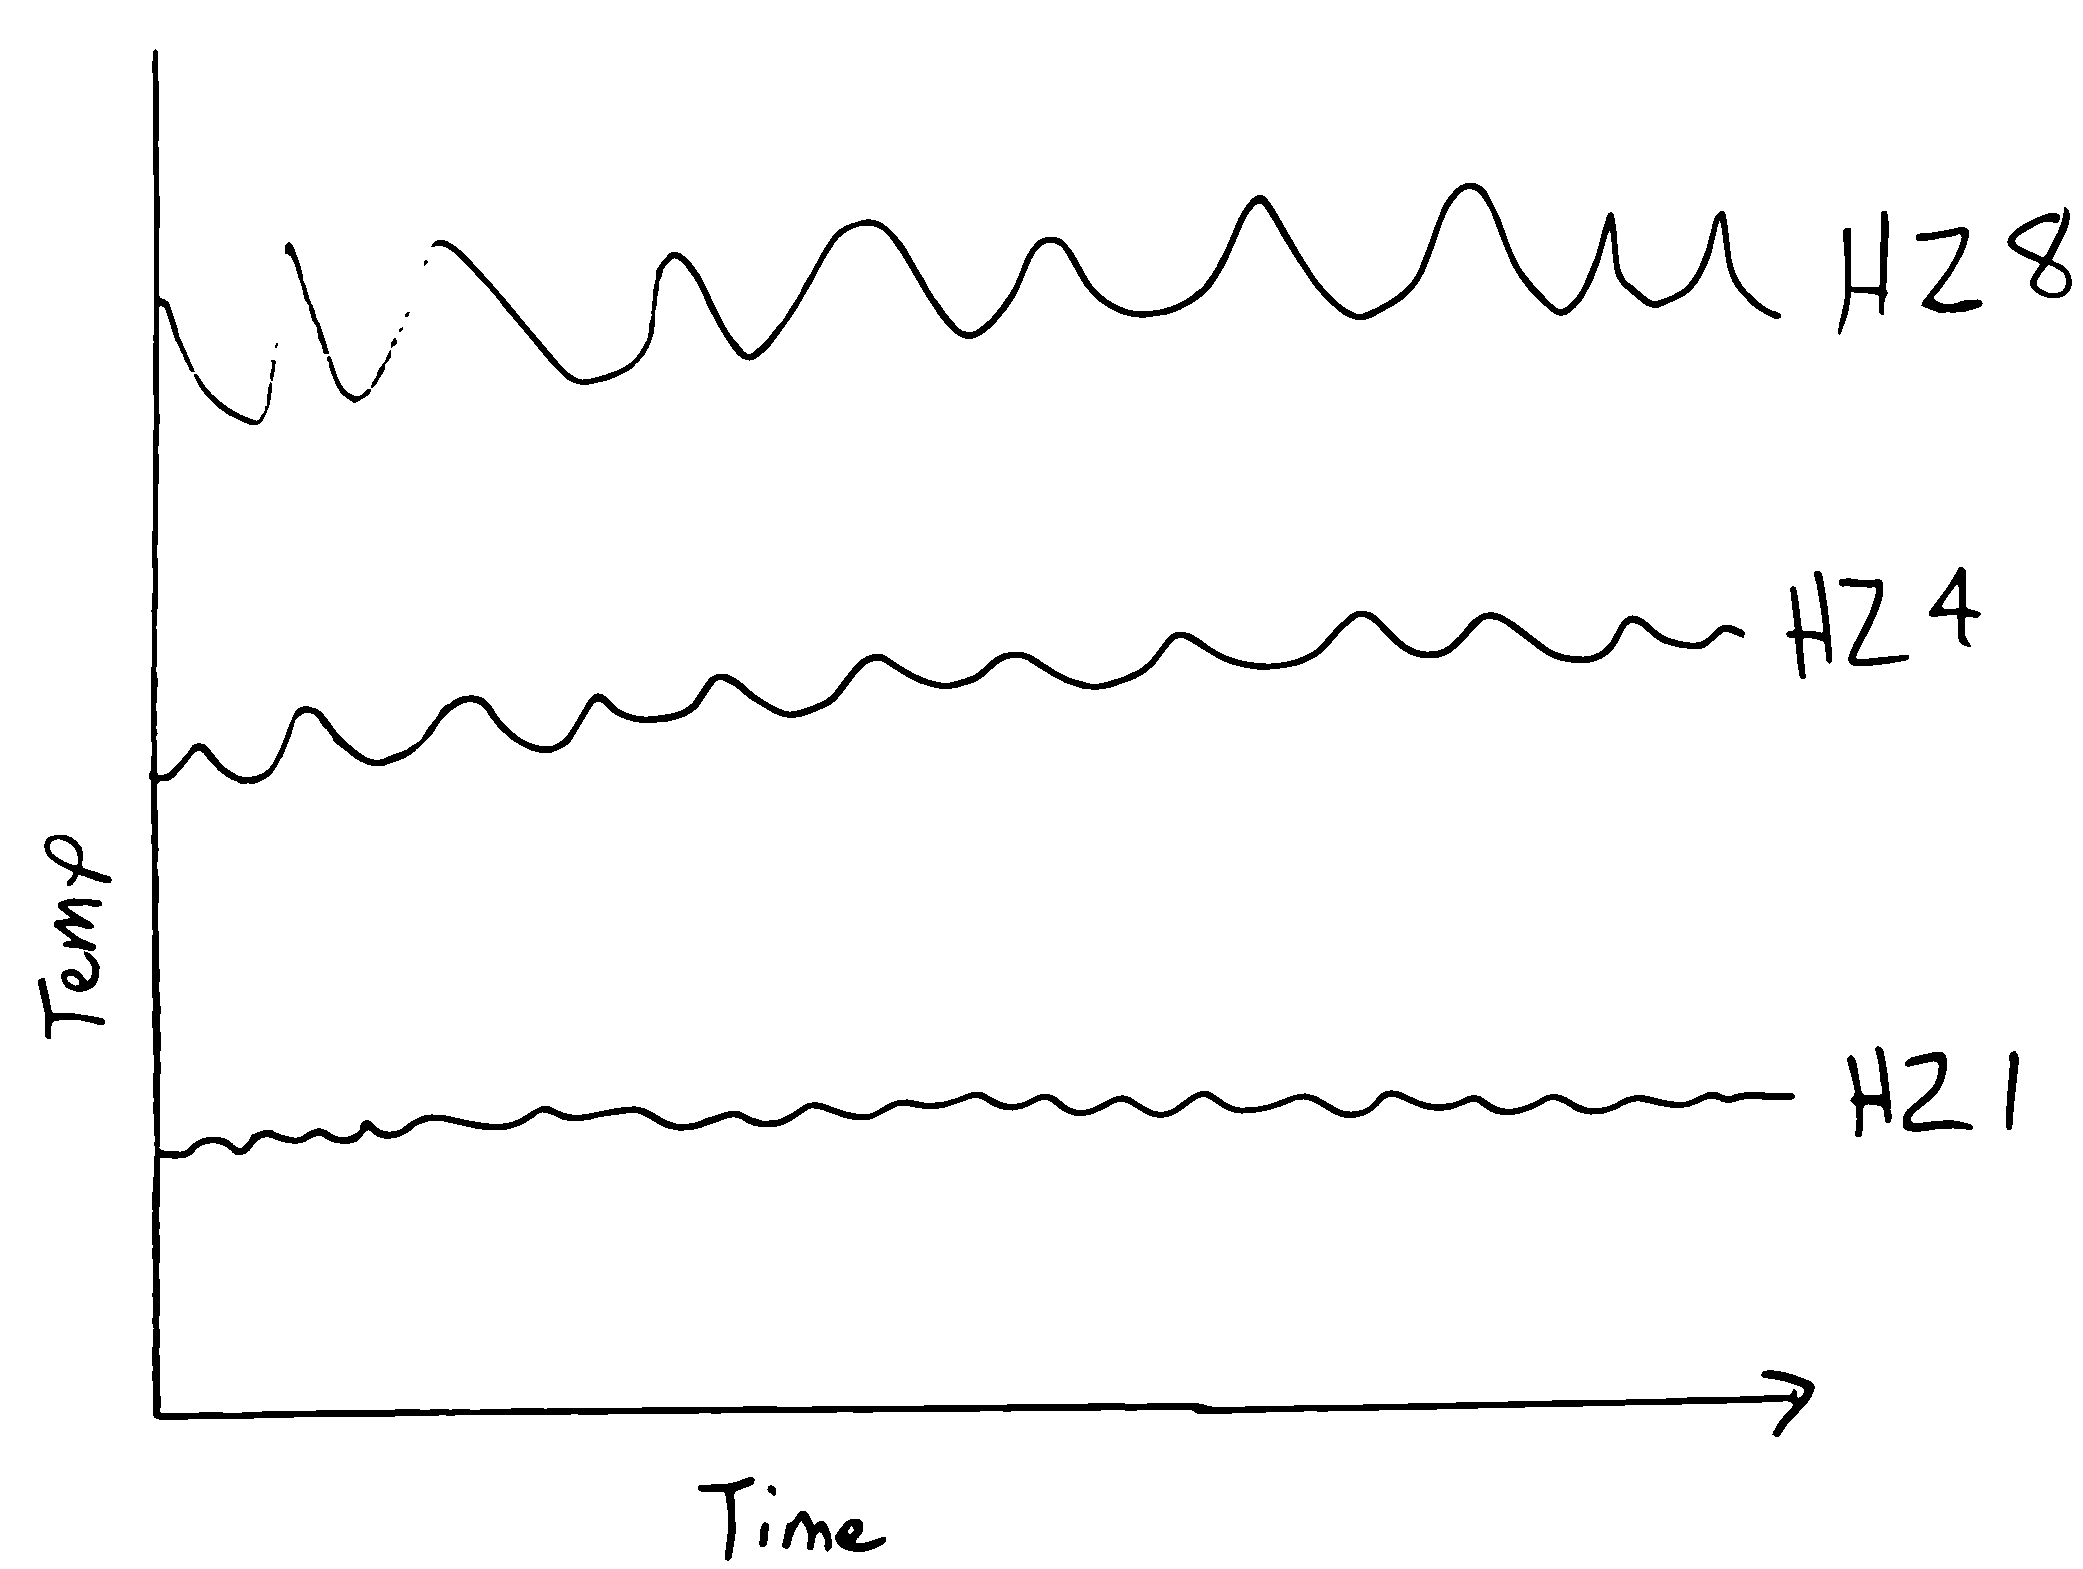
\includegraphics[width=\textwidth]{../diagrams/temp/noise.pdf}
\caption{Comparison of noise levels at the \mlx' various sampling speeds}
\label{fig:noise}
\end{figure}

\begin{figure}
\centering
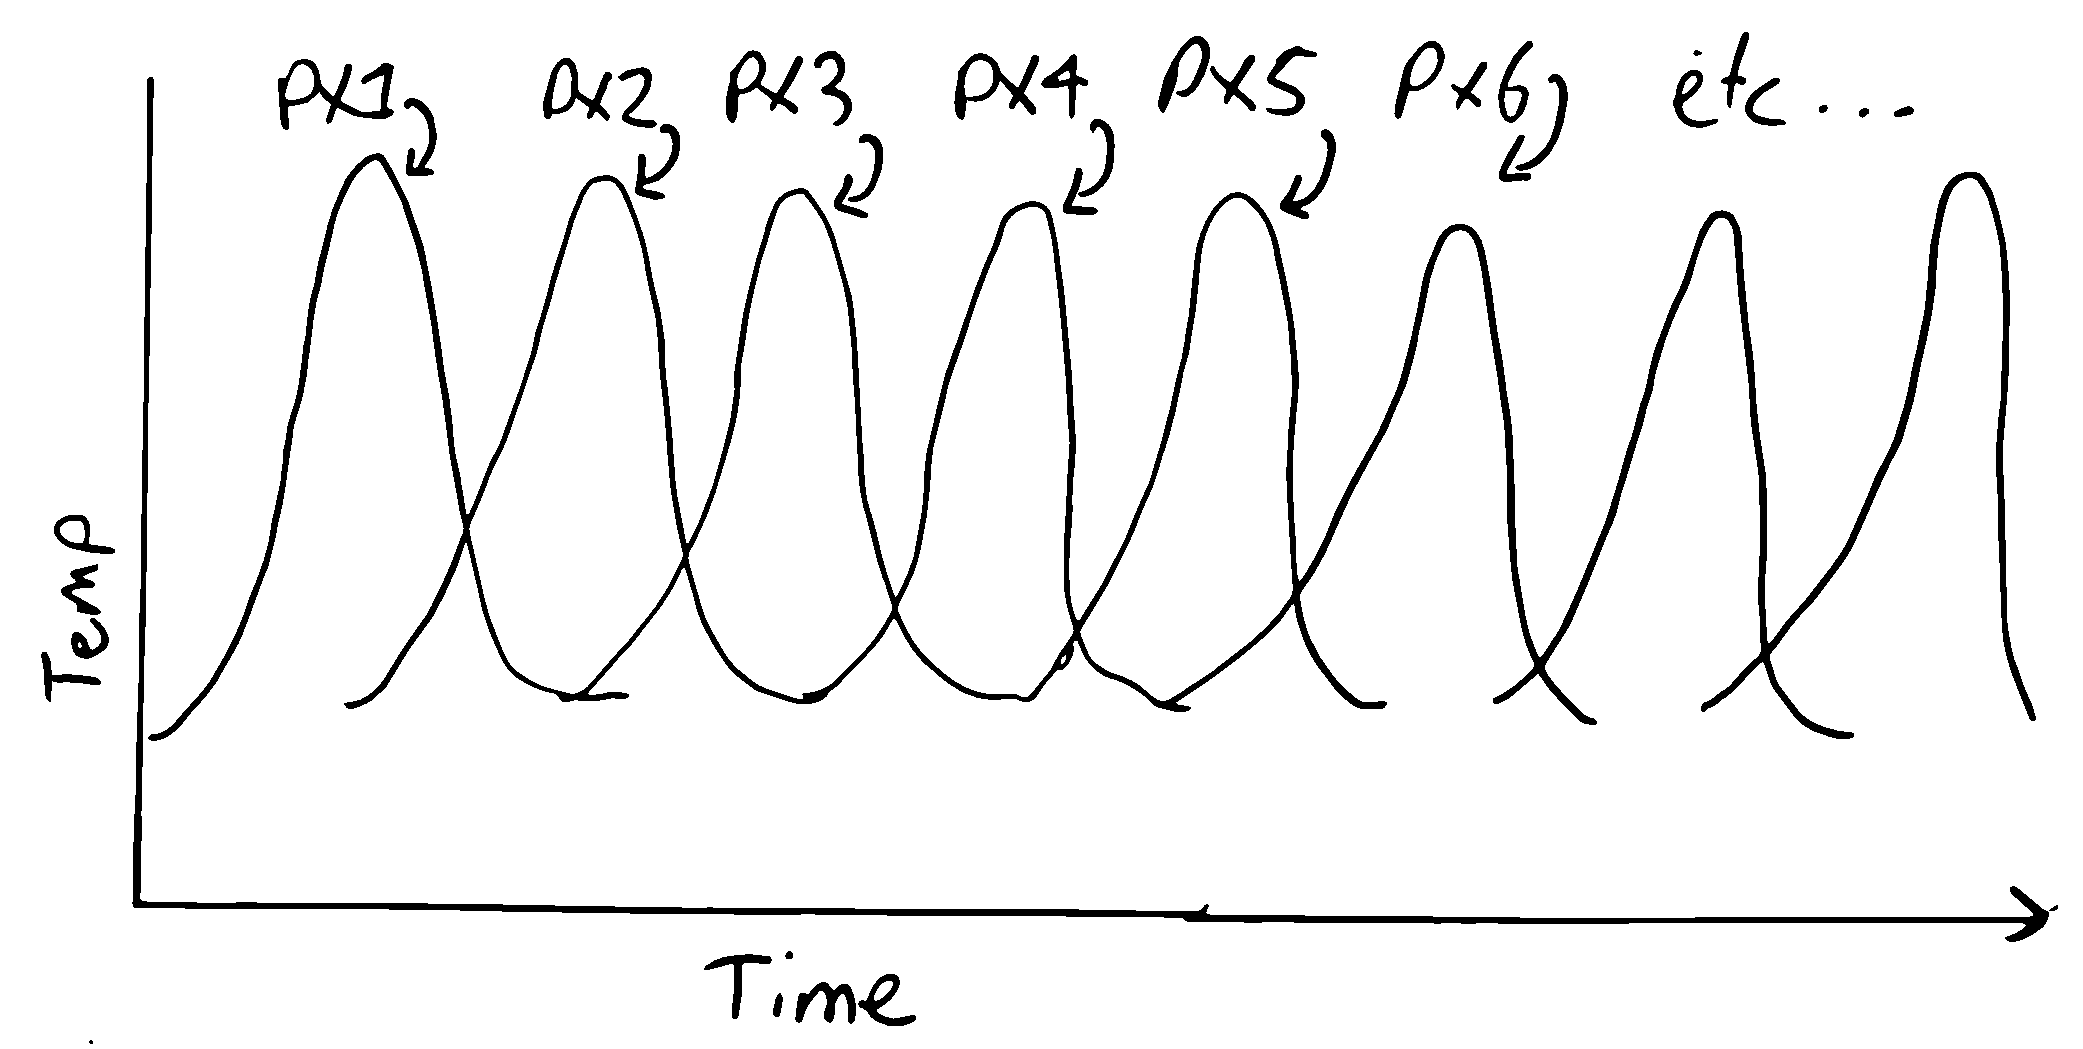
\includegraphics[width=\textwidth]{../diagrams/temp/motion.pdf}
\caption{Different \mlx pixel temperature values as hot object moves across row}
\label{fig:hotmotion}
\end{figure}

\begin{figure}
\centering
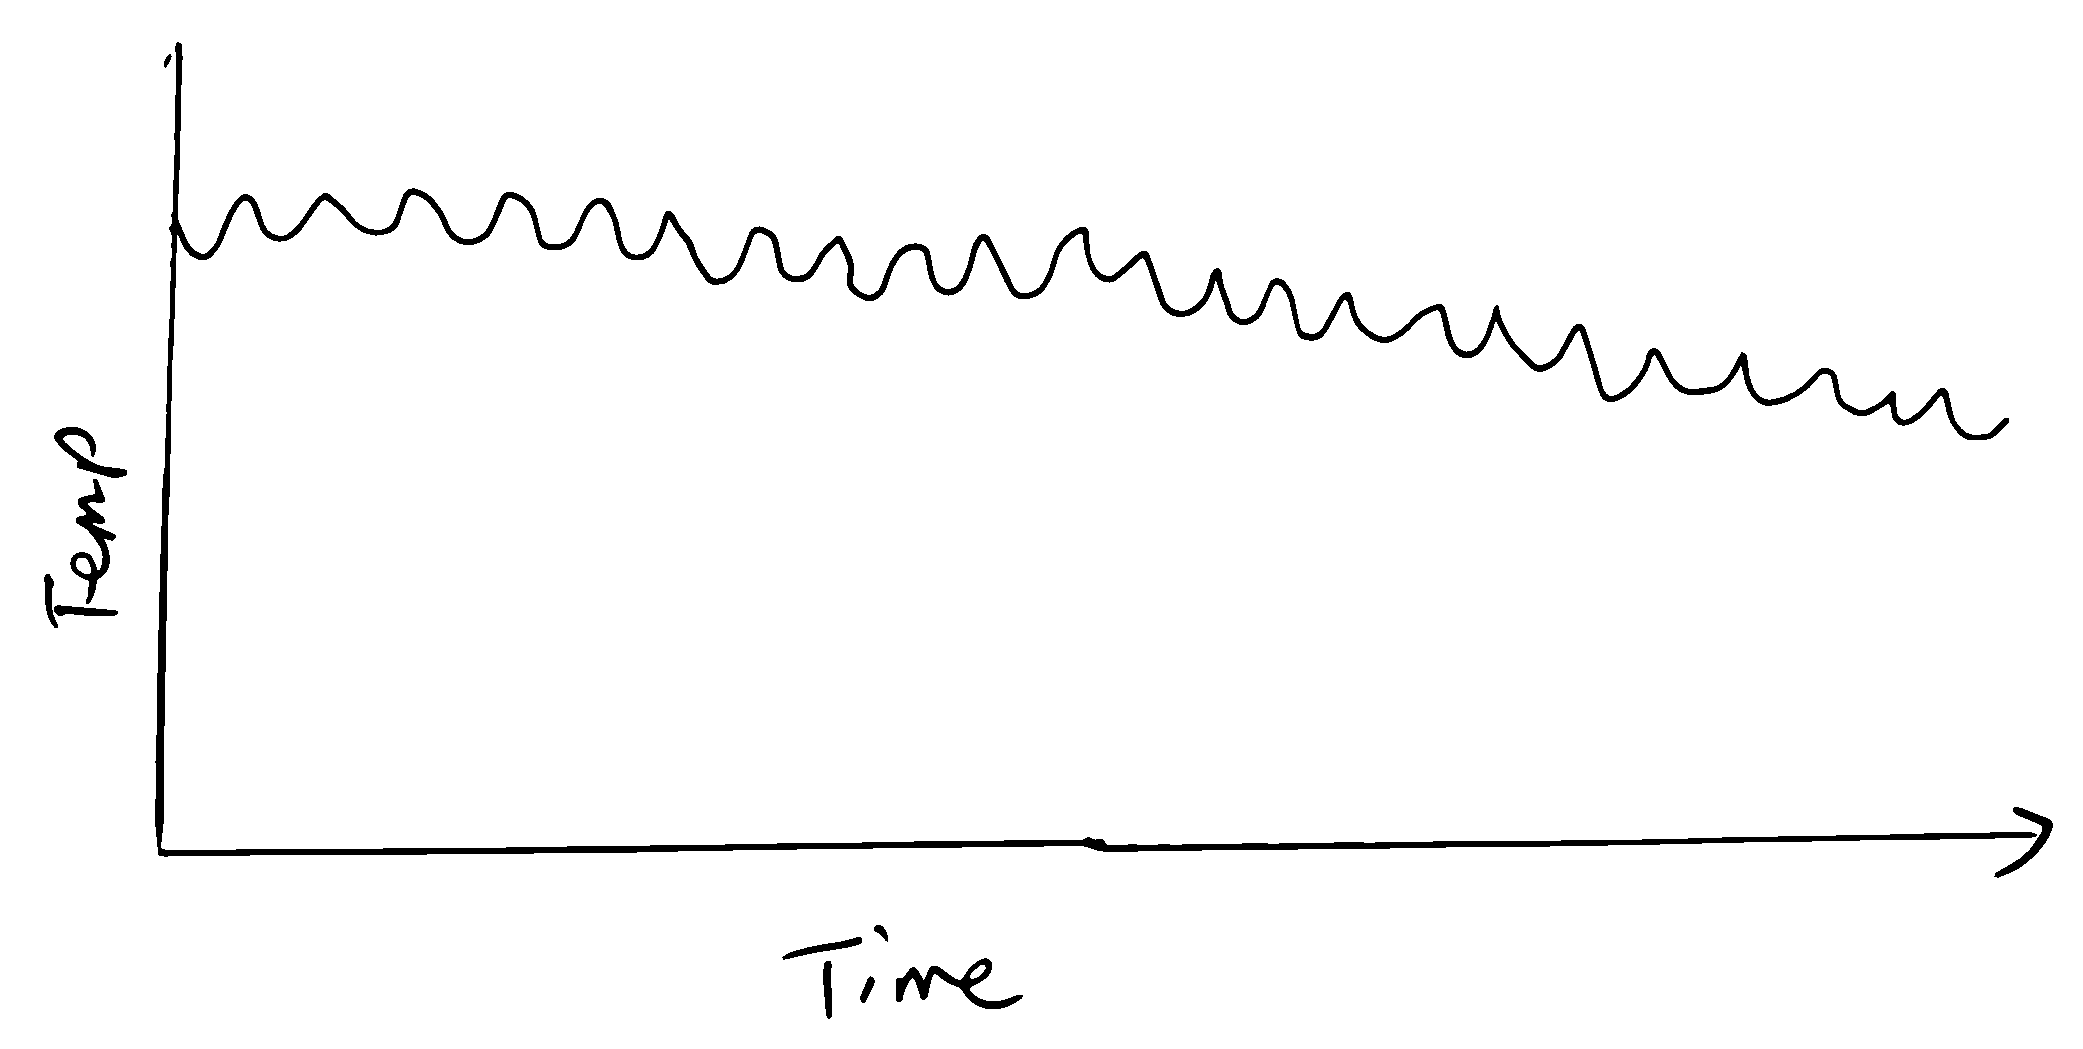
\includegraphics[width=\textwidth]{../diagrams/temp/cooldown.pdf}
\caption{Variation in temperature detected for hot object at 1Hz sampling ration}
\label{fig:cooldown}
\end{figure}
 
 \ifcsdef{mainfile}{}{\bibliography{../references/primary}}
\end{document}
